\section{Cobalt}

 The KE cutoff of ccECP-soft Co is about 700 Ry. Below is the atomic gaps and molecular transferability test. Original published ccECP is included there as comparison too.

Note that here I have an ECP labeled as 600Ry, this is generated by Cody using Opium package from Troullier-Martins method fitting from original ccECPs. It is a numerical ECP but I fit it into Gaussian and test it in atomic gaps and molecules. The fit is not perfect and can not represent the full accuracy of it.

The Co ccECP-soft parameter is give below and can also be downloaded under ./ccECP-soft-param/ directory:\\
17 3  \\
2 2 4 \\
2 10.013765  15.836729    \\ 
2 15.026211  172.58644    \\
2 7.9885909 15.3494954    \\
2 14.997586  90.995647    \\
1 12.003882  17.0    \\
3 10.005064  204.06599    \\
2 9.4548033 -117.74448    \\
2 6.0069244 2.85018517    \\


\begin{figure*}[!htbp]
\centering
\begin{subfigure}{0.5\textwidth}
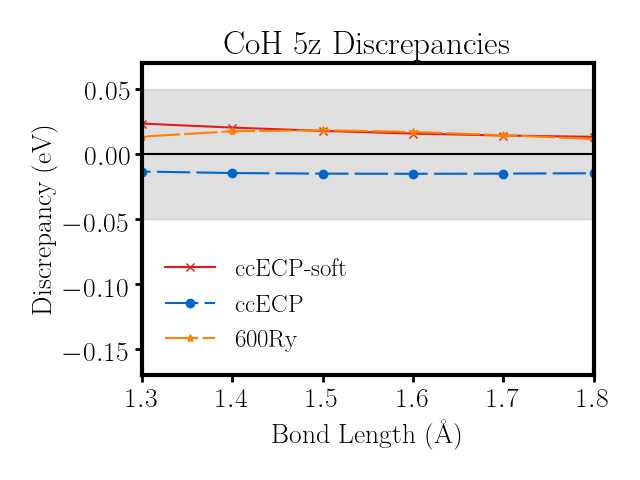
\includegraphics[width=\textwidth]{figures/CoH_5z.png}
\caption{CoH 5Z binding curve discrepancies}
\label{fig:CoO_5z}
\end{subfigure}%
\begin{subfigure}{0.5\textwidth}
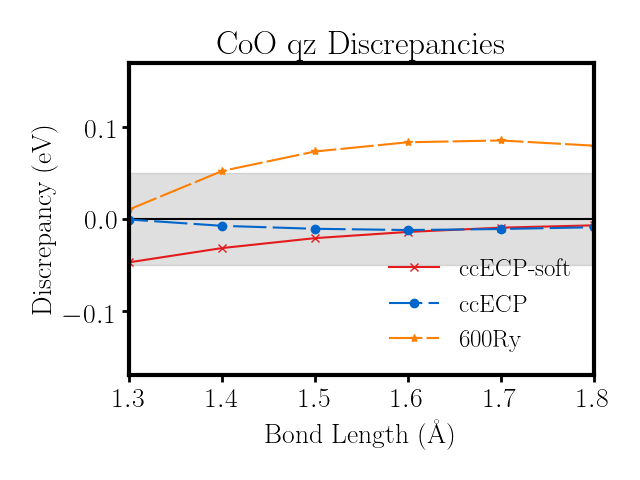
\includegraphics[width=\textwidth]{figures/CoO_qz.png}
\caption{CoO QZ binding curve discrepancies}
\label{fig:CoO_qz}
\end{subfigure}
\caption{Binding energy discrepancies for (a) CoH 5Z and (b) CoO QZ molecules with regard to CCSD(T). The shaded region indicates the band of chemical accuracy. }%The dashed vertical line represents the equilibrium geometry.}
\label{fig:Co_mols}
\end{figure*}



\begin{table*}[!htbp]
\setlength{\tabcolsep}{3pt} %% default is 6pt
\centering
\caption{Co gaps and relative errors for various ECPs.  All values in eV}
\resizebox{0.5\textwidth}{!}{%
\begin{tabular}{ll|cccccccccr}
\hline\hline
States and Symmetry &   &   AE &        ccECP   &   ccECP-soft   &  600Ry  \\
\hline
{[Ar] $3d^84s^2$ }    EA  & $^3F$ & -0.648825 & -0.011727 &   0.023771 &  0.017302  \\
{[Ar] $3d^84s^1$ }        & $^4F$ &  0.404998 & -0.018725 &   0.010404 & -0.022794  \\
{[Ar] $3d^9$ }            & $^2D$ &   3.29022 & -0.028436 &   0.018581 &  0.053097  \\
{[Ar] $3d^74s^1$ }        & $^5F$ &    8.2851 & -0.014988 &  -0.025523 & -0.006439  \\
{[Ar] $3d^8$ }            & $^3F$ &   7.85217 & -0.013046 &  -0.004582 & -0.038360  \\
{[Ar] $3d^7$ }  2nd Ion   & $^4F$ &   24.9596 &  0.005217 &  -0.024421 &  0.062209  \\
{[Ar] $3d^6$ }  3rd Ion   & $^5D$ &   58.4749 &  0.009923 &  -0.040255 &  0.461901  \\
\hline
MAD & &                                     &  0.014580 &   0.021077   &  0.094586  \\
\hline
\hline
\end{tabular}
}
\end{table*}